
\graphicspath{{./FiguresA/}}
\chapter{Evaluación de Diferentes Arquitecturas de Control para Teleoperación}
\label{ch:arquitecturas}
El objetivo de este capítulo es comprobar de manera experimental los principales algoritmos de control bilateral así como sus ventajas e inconvenientes.

\begin{figure}[htbp]
\centering
	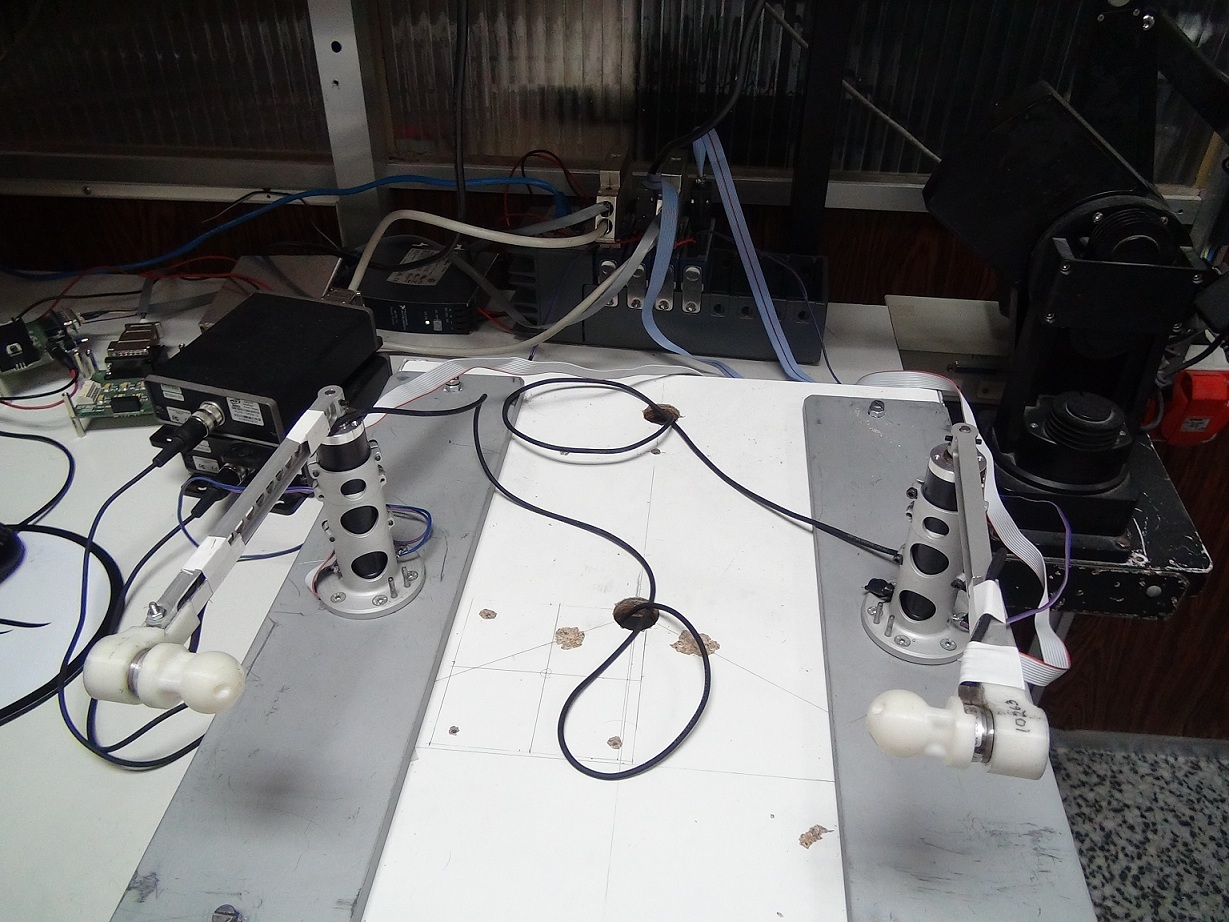
\includegraphics[scale=0.2]{setup.jpg}
	\caption{Fotografía de la plataforma experimental}
  	\label{fig:setup}
\end{figure}
Este trabajo se ha desarrollado en la plataforma experimental mostrada en la figura \ref{fig:setup}, donde la implementación de los algoritmos se realiza utilizando el entorno de desarrollo LABVIEW.\\
Los elementos principales de la plataforma experimental son:
\begin{itemize}
\item 2 x Motor Maxon, serie RE 25, reductor planetario GP 26 B (1:104), encoder MR.
\item 1 x Controlador compact RIO 9022 dotado de una FPGA.
\item 2 x NI 9505 Módulo de Drive Servo de DC de Escobillas con Puente H Completo.
\item 2 x NI 9205 Módulo de Entrada Analógica de 32 Canales.
\end{itemize}

El modelo de ambos motores, maestro y esclavo, que se ha utilizado es el siguiente:
\begin{eqnarray}
\dfrac{\theta(s)}{I(s)} &=& \dfrac{A}{(J s^2+B s)} = \dfrac{4.5552}{0.0118s^2 + 2.8607s} \\[0.5cm]
F \cdot 0.16 &=& R_T K_\tau I \nonumber
\label{eq:model}
\end{eqnarray}
Donde,
\begin{itemize}
\item $F$ es la fuerza aplicada al dispositivo.
\item $R_T$ es el factor de reducción de los motores e igual a 104.
\item $K_\tau$ es la constante de par de los motores e igual a $43.8\cdot 10^{-3} \frac{Nm}{A}$.
\item $I$ es la intensidad que fluye por los motores. Máximo 0.7 A.
\end{itemize}
\begin{figure}[htbp]
\centering
	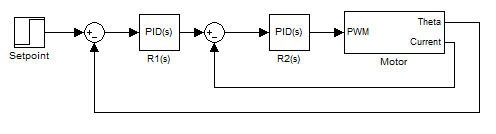
\includegraphics[scale=0.5]{cascada}
	\caption{Diagrama de bloques del control implementado en cada motor} % labelInTOC
  	\label{fig:cascada} %% label for entire figure
\end{figure}
Otro aspecto a tener en cuenta es el tipo de control implementando en cada motor ya que con el objetivo de protegerlos se utiliza un esquema en cascada como se muestra en la figura \ref{fig:cascada}. Para los propósitos de este trabajo solo se ha considerado el regulador $R_1(s)$ ya que el lazo interno responde más rápido (hasta 10 veces más rápido) y se puede considerar únicamente su valor en régimen permanente, la unidad, ya que $R_2(s)$ es un regulador PI (error nulo en régimen permanente).
\begin{figure}[htbp]
\centering
	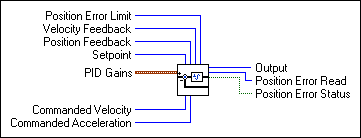
\includegraphics[scale=0.6]{fixedPointPID}
	\caption{Fixed Point PID VI} 
  	\label{fig:fixedPID}
\end{figure}
Con respecto a $R_1(s)$ cabe mencionar que se ha utilizado el VI mostrado en la figura \ref{fig:fixedPID}. Este PID permite gran flexibilidad ya que se pueden probar reguladores clásicos así como versiones mejoradas en las que se considera la velocidad o aceleración del motor. En la figura \ref{fig:pidloop} se muestra de manera gráfica como se relacionan los diferentes parámetros y ganancias con las que cuenta el VI en cuestión.
\begin{figure}[htbp]
\centering
	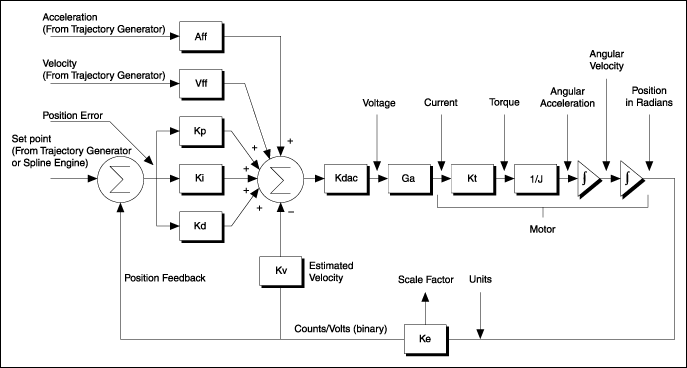
\includegraphics[scale=0.5]{pidloop} 
	\caption{NI SoftMotion Control Loop} 
  	\label{fig:pidloop} 
\end{figure}

\section{Control Posición - Posición}
\label{sec:pos-pos}
En esta sección se realiza en primer lugar un análisis teórico de la estabilidad y de la percepción por parte del operador en este tipo de algoritmo en sus casos extremos:
\begin{itemize}
\item Espacio libre: La impedancia del entorno es nula ($K_e = 0$), el esclavo se mueve libremente, y la única fuerza externa que actúa sobre el sistema es la del operador sobre el maestro.
\item Contacto con un objeto rígido: El esclavo esta en contacto con un entorno rígido ideal ($K_e = \infty$).
\end{itemize}
Posteriormente se presentaran algunos resultados obtenidos en la plataforma experimental.
\begin{figure}[htbp]
\centering
	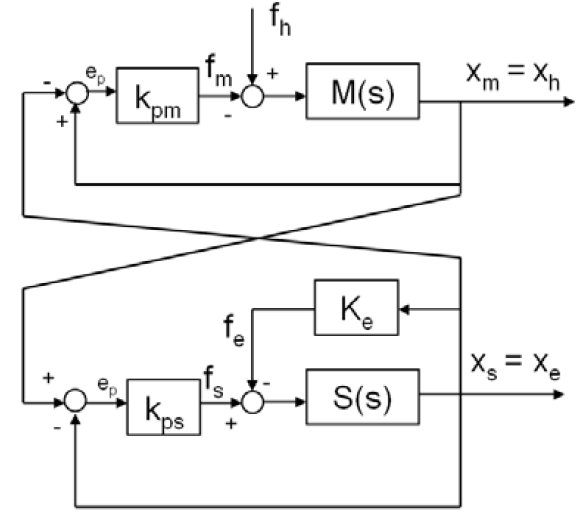
\includegraphics[scale=0.5]{pos-pos}
	\caption{Arquitectura de control Posición - Posición} % labelInTOC
  	\label{fig:pos-pos} %% label for entire figure
\end{figure}

En la figura \ref{fig:pos-pos} se muestra la arquitectura en cuestión. Con el fin de analizar los casos extremos y como serán percibidos por el operador es necesario simplificar este diagrama de bloques reemplazando el valor de $K_e$.
\begin{figure}[htbp]
\centering
	\begin{subfigure}[h]
		\centering
		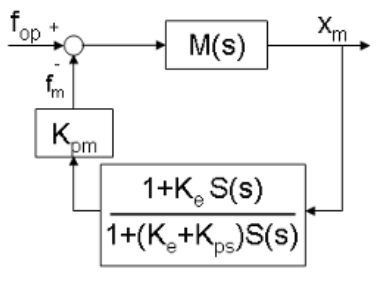
\includegraphics[scale=0.5]{pos-pos-operator}
		\caption{Esquema visto desde el maestro}
	\end{subfigure}
	\begin{subfigure}[h]
		\centering
		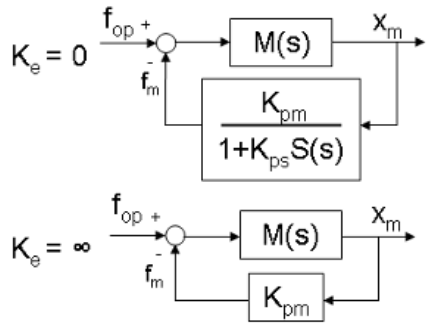
\includegraphics[height=4cm]{pos-pos-kvalues}
		\caption{Casos extremos}
    \end{subfigure}
	\caption{Diagrama de bloques para los casos extremos del control Posición - Posición}
  	\label{fig:pos-pos-casos}
\end{figure}

En la figura \ref{fig:pos-pos-casos} se muestran los diagramas simplificados así como las funciones de transferencia resultantes en los casos extremos.
\\
No es necesario entrar en el detalle de los modelos del maestro y esclavo para intuir la percepción por parte del operador:
\begin{itemize}
\item $K_e = 0$: $H(s)$ esta dada por $\frac{K_{pm}}{1+K_{ps}S(s)}$ con lo cual el operador percibirá cierta fuerza a pesar de que ninguna fuerza se esta ejerciendo sobre el esclavo.
\item $K_e = \infty$: $H(s)$ esta dada por $K_{pm}$ con lo cual la máxima impedancia que percibirá el operador esta determinada por el regulador (P, PD, etc.) del maestro ($K_{pm}$).
\end{itemize}

En lo que concierne a la estabilidad de este sistema se puede analizar también en los casos extremos. En aras de la sencillez se considerará el caso en que los dos reguladores $K_{pm}$ y $K_{ps}$ son proporcionales.
Retomando el modelo del sistema de la ecuación \eqref{eq:model} y aplicando la relación para expresarlo en función de la fuerza tenemos:
\begin{equation}
G(s) = \dfrac{\theta(s)}{F(s)} = \dfrac{4.5552}{0.0118s^2 + 2.8607s}\cdot \dfrac{0.16}{R_tK_t} = \dfrac{0.16}{0.0118 s^2 + 2.861 s}
\end{equation}
\begin{itemize}
\item $K_e = 0$:
\begin{equation}
G_r(s) = \dfrac{M(s)}{1 + M(s)\dfrac{K_{pm}}{1 + K_{ps}S(s)}} = \dfrac{0.16}{0.0118 s^2 + 2.861 s + 0.16(K_{pm} + K_{ps})}
\end{equation}
\begin{table}[htbp]
  \centering
  \caption{Tabla del criterio de Routh-Hurwitz para $K_e = 0$ (Posición - Posición)}
    \begin{tabular}{ccc}
    \toprule
    $s_2$	& $0.0118$		& $0.16(K_{pm} + K_{ps})$ \\
    $s_1$	& $2.861$		& 	\\
 	$s_0$	& $0.16(K_{pm} + K_{ps})$		& 	\\
    \bottomrule
    \end{tabular}
  \label{tab:routh-pos-pos0}
\end{table}
Donde $G_r(s)$ es la función de transferencia en lazo cerrado. Aplicando el criterio de estabilidad de Routh-Hurwitz (Tabla \ref{tab:routh-pos-pos0}), el cual establece que para que el sistema sea estable no deben presentarse cambios de signo en la primer columna, se comprueba que el sistema es estable para todos los valores \textbf{positivos} de $K_{pm}$ y $K_{ps}$.

\item $K_e = \infty$:
\begin{equation}
G_r(s) = \dfrac{M(s)}{1 + M(s)\dfrac{K_{pm}}{1 + K_{ps}S(s)}} = \dfrac{0.16}{0.0118 s^2 + 2.861 s + 0.16K_{pm}}
\end{equation}
\begin{table}[htbp]
  \centering
    \caption{Tabla del criterio de Routh-Hurwitz para $K_e = \infty$ (Posición - Posición)}
    \begin{tabular}{ccc}
    \toprule
    $s_2$	& $0.0118$		& $0.16K_{pm}$ \\
    $s_1$	& $2.861$		& 	\\
 	$s_0$	& $0.16K_{pm}$		& 	\\
    \bottomrule
    \end{tabular}%
  \label{tab:routh-pos-pos1}%
\end{table}%
Aplicando el criterio de estabilidad de Routh-Hurwitz (Tabla \ref{tab:routh-pos-pos1}) se comprueba que el sistema es estable para todos los valores \textbf{positivos} de $K_{pm}$.
\end{itemize}

\subsection{Simulación del Sistema}
\label{sub:pos-pos-sim}
Con el fin de comprobar el funcionamiento del sistema se ha diseñado un regulador PD para controlar tanto al maestro ($K_{pm}$) como el esclavo ($K_{ps}$). Se podría pensar que el regulador PID sería una mejor opción, pero la acción integral no es recomendable por varias razones, entre ellas las siguientes:
\begin{itemize}
\item La intención no es sólo que el regulador fuerce al sistema a ir a la posición deseada, sino que también refleje las fuerzas de la forma más clara y real posible. Con este fin, no tiene ningún sentido que ante un error de posición constante, la salida de nuestro controlador aumente y con ello aumenten las fuerzas que se representan en el maestro, tiene más sentido que estas sean constantes pues las fuerzas a las que esta sometido el esclavo en este caso particular son constantes.
\item Al ser un proceso con gran cantidad de no linealidades (p. ej. los choques del esclavo contra el entorno) habría que incluir un Wind-Up, ya que si no se controla la acción integral se perjudicaría mucho el sistema.
\end{itemize}
Para el diseño del regulador se ha considerado cada motor de manera independiente y dado que son idénticos se tiene:
\begin{equation}
M(s) = S(s) = \dfrac{\theta(s)}{F(s)} = \dfrac{0.16}{0.0118 s^2 + 2.861 s}
\label{eq:force-motor-model}
\end{equation}
Teniendo en cuenta que el tiempo de muestreo es $T = 1$ ms, la ecuación \eqref{eq:force-motor-model} se discretiza como:
\begin{equation}
M(z) = S(z) = \dfrac{\theta(z)}{F(z)} = \dfrac{6.2634\cdot 10^{-6}(z+0.9224)}{(z-1)(z-0.7847)}
\end{equation}
Utilizando la \mcode{rtool} de MATLAB y definiendo las siguientes especificaciones:
\begin{equation*}
M_p \leq 10\% \quad t_s \leq 50 \mbox{ms} \quad e_p = 0
\end{equation*}
Se ha diseñado un regulador PD que permitirá controlar en posición cada motor. En la figura \ref{fig:pos-pos-reg} se muestra el lugar de las raíces resultante así como la respuesta del sistema en lazo cerrado ante entrada escalón unitario.
\begin{figure}[htbp]
\centering
	\begin{subfigure}[h]
		\centering
		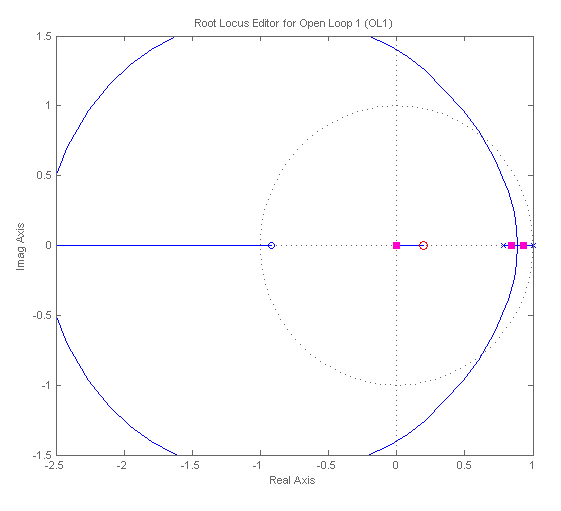
\includegraphics[height=5.25cm]{pos-pos-rlocus}
		\caption{Lugar de las raíces}
	\end{subfigure}
	\begin{subfigure}[h]
		\centering
		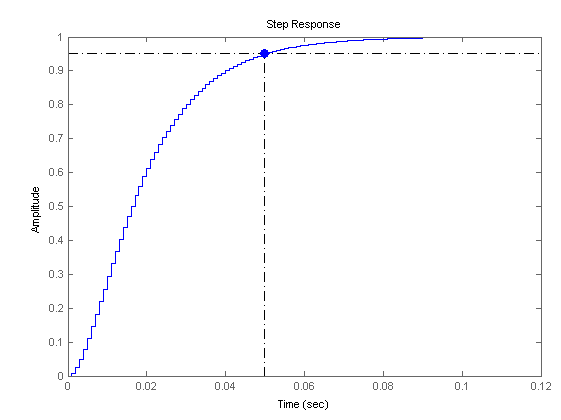
\includegraphics[height=5.25cm]{pos-pos-step}
		\caption{Respuesta ante entrada escalón unitario}
    \end{subfigure}
	\caption{Respuesta del PD diseñado para control en posición de cada motor}
  	\label{fig:pos-pos-reg}
\end{figure}

La función de transferencia de dicho regulador es:
\begin{equation}
R(z) = \dfrac{K(z-c_d)}{z} = \dfrac{1100(z-0.2)}{z}
\label{eq:regulador}
\end{equation}
Se ha comprobado el funcionamiento del sistema en su conjunto en el modelo de SIMULINK que se muestra en la figura \ref{fig:pos-pos-esq}.
\begin{figure}[htbp]
\centering
	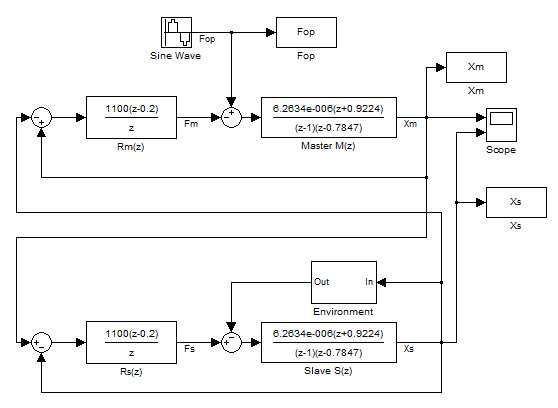
\includegraphics[width=10cm]{pos-pos-esq}
	\caption{Esquema de control Posición - Posición en Simulink}
  	\label{fig:pos-pos-esq}
\end{figure}
En la figura \ref{fig:pos-pos-sim} se muestran los resultados obtenidos para los casos extremos que se han planteado.
\begin{figure}[htbp]
\centering
	\begin{subfigure}[h]
		\centering
		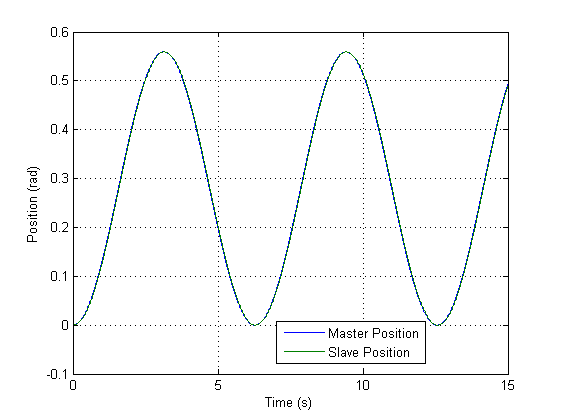
\includegraphics[height=5.25cm]{pos-pos-libre}
		\caption{$K_e = 0$, entrada sinusoidal}
	\end{subfigure}
	\begin{subfigure}[h]
		\centering
		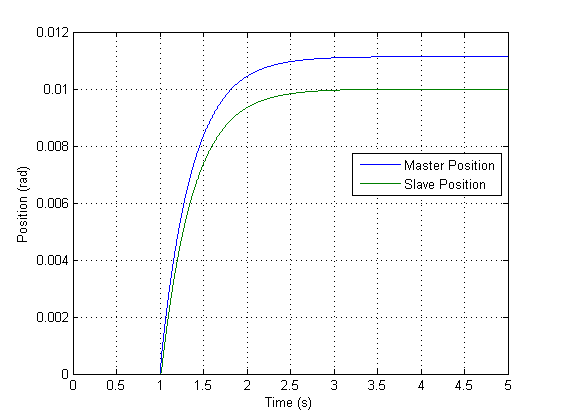
\includegraphics[height=5.25cm]{pos-pos-env}
		\caption{Respuesta ante entrada escalón unitario}
    \end{subfigure}
	\caption{Simulación del control Posición - Posición}
  	\label{fig:pos-pos-sim}
\end{figure}

\subsection{Experimentos}
\label{sub:pos-pos-exp}
\begin{figure}[htbp]
\centering
	\begin{subfigure}[h]
		\centering
		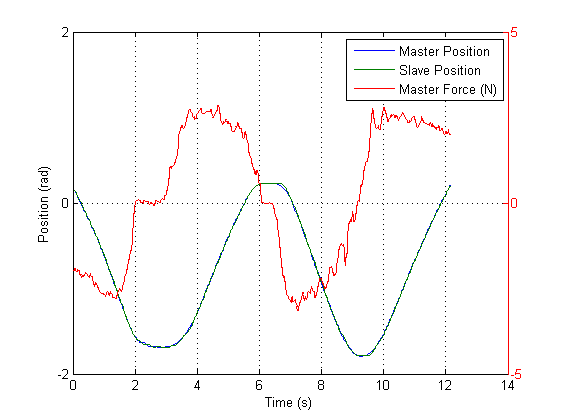
\includegraphics[height=5.25cm]{pos-pos-exp-libre}
		\caption{Movimiento libre}
		\label{fig:pos-pos-exp-libre}
	\end{subfigure}
	\hspace{0.1cm}
	\begin{subfigure}[h]
		\centering
		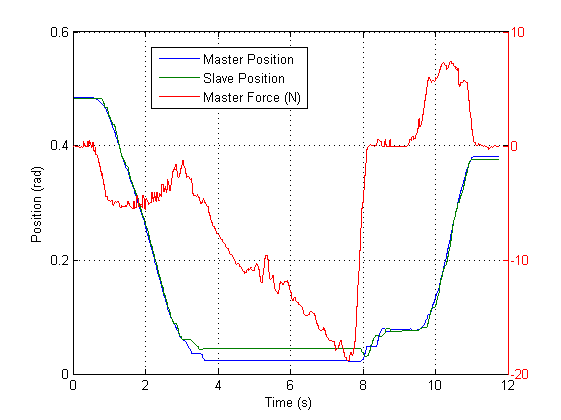
\includegraphics[height=5.25cm]{pos-pos-exp-env}
		\caption{Colisión contra objeto rígido (t $\simeq$ 4-8 s.)}
		\label{fig:pos-pos-exp-env}
    \end{subfigure}
	\caption{Resultados experimentales del control Posición - Posición}
  	\label{fig:pos-pos-exp}
\end{figure}

Con el regulador diseñado se han realizado experimentos para comprobar el funcionamiento del sistema.
\begin{itemize}
\item Movimiento libre: En la figura \ref{fig:pos-pos-exp-libre} se muestra como en el movimiento libre el maestro y el esclavo tienen la misma posición con error prácticamente nulo. Respecto a la fuerza percibida por el operador se aprecia que a pesar de estar en movimiento libre es necesario realizar hasta 3N para modificar la posición del sistema.
\item Colisión: En la figura \ref{fig:pos-pos-exp-env} se puede observar como durante el periodo de tiempo comprendido entre 4 y 8 segundos hay un error significativo en la posición. Además por la lectura de fuerza se puede ver que el pico de fuerza realizado por el operador alcanza los -19 Newtons.
\end{itemize}

\section{Control Fuerza - Posición}
\label{sec:force-position}
En esta sección se realiza en primer lugar un análisis teórico de la estabilidad y de la percepción por parte del operador en este tipo de algoritmo en sus casos extremos:
\begin{itemize}
\item Espacio libre: La impedancia del entorno es nula ($K_e = 0$), el esclavo se mueve libremente, y la única fuerza externa que actúa sobre el sistema es la del operador sobre el maestro.
\item Contacto con un objeto rígido: El esclavo esta en contacto con un entorno rígido ideal ($K_e = \infty$).
\end{itemize}
Posteriormente se presentaran algunos resultados obtenidos en la plataforma experimental.
\begin{figure}[htbp]
\centering
	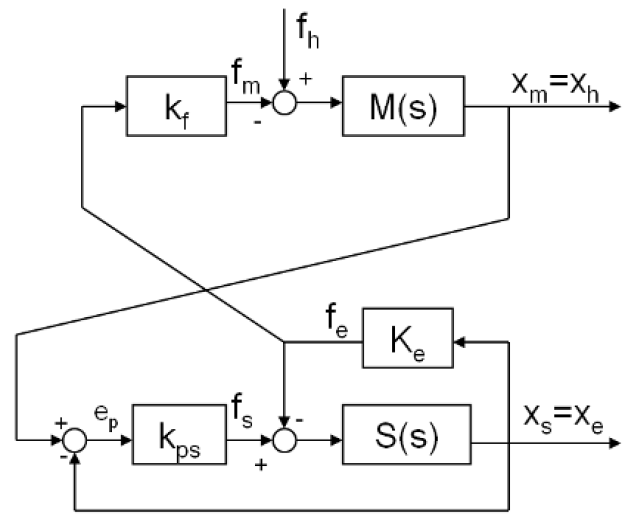
\includegraphics[height=8cm]{force-pos}
	\caption{Arquitectura de control Fuerza - Posición}
  	\label{fig:force-pos} 
\end{figure}
En la figura \ref{fig:force-pos} se muestra la arquitectura en cuestión. Con el fin de analizar los casos extremos y como serán percibidos por el operador es necesario simplificar este diagrama de bloques reemplazando el valor de $K_e$.
\begin{figure}[htbp]
\centering
	\begin{subfigure}[h]
		\centering
		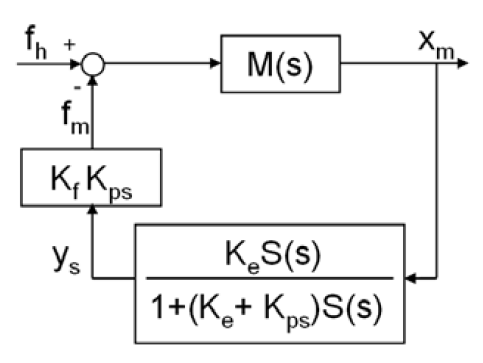
\includegraphics[height=4cm]{force-pos-operator}
		\caption{Esquema visto desde el maestro}
	\end{subfigure}
	\begin{subfigure}[h]
		\centering
		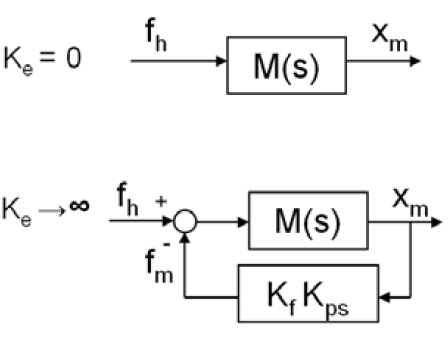
\includegraphics[height=4cm]{force-pos-kvalues}
		\caption{Casos extremos}
    \end{subfigure}
	\caption{Diagrama de bloques para los casos extremos del control Fuerza - Posición}
  	\label{fig:force-pos-casos}
\end{figure}

En la figura \ref{fig:force-pos-casos} se muestran los diagramas simplificados así como las funciones de transferencia resultantes en los casos extremos.
\\
No es necesario entrar en el detalle de los modelos del maestro y esclavo para intuir la percepción por parte del operador:
\begin{itemize}
\item $K_e = 0$: No hay $H(s)$. Con lo cual el operador no percibirá ninguna fuerza por la interacción con el entorno sino solamente las inherentes a la masa e inercia del maestro (dinámica del maestro $M(s)$).
\item $K_e = \infty$: $H(s)$ esta dada por $K_{f}K_{ps}$ con lo cual la máxima impedancia que percibirá el operador esta determinada por el regulador (P, PD, etc.) del esclavo ($K_{ps}$) y el factor con el que se refleja la fuerza $K_{f}$.
\end{itemize}

En lo que concierne a la estabilidad de este sistema se puede analizar también en los casos extremos. En aras de la sencillez se considerará el caso en que el regulador $K_{ps}$ y el factor $K_{f}$ son proporcionales.
Retomando el modelo del sistema de la ecuación \eqref{eq:model} y aplicando la relación para expresarlo en función de la fuerza tenemos:
\begin{equation}
G(s) = \dfrac{\theta(s)}{F(s)} = \dfrac{4.5552}{0.0118s^2 + 2.8607s}\cdot \dfrac{0.16}{R_tK_t} = \dfrac{0.16}{0.0118 s^2 + 2.861 s}
\end{equation}
\begin{itemize}
\item $K_e = 0$: Tenemos un lazo abierto de un sistema que es estable, y por lo tanto tendremos una salida acotada.

\item $K_e = \infty$: La ecuación en del sistema realimentado será:
\begin{equation}
G_r(s) = \dfrac{M(s)}{1 - M(s)K_{ps}K_f} = \dfrac{0.16}{0.0118 s^2 + 2.861 s + 0.16(K_f+K_{ps})}
\end{equation}
\begin{table}[htbp]
  \caption{Tabla del criterio de Routh-Hurwitz para $K_e = \infty$ (Fuerza - Posición)}
  \centering
    \begin{tabular}{ccc}
    \toprule
    $s_2$	& $0.0118$		& $0.16(K_f+K_{ps})$ \\
    $s_1$	& $2.861$		& 	\\
 	$s_0$	& $0.16(K_f+K_{ps})$		& 	\\
    \bottomrule
    \end{tabular}
  \label{tab:force-pos-routh}
\end{table}
Aplicando el criterio de estabilidad de Routh-Hurwitz (Tabla \ref{tab:force-pos-routh}) se comprueba que el sistema es estable para todos los valores \textbf{positivos} de $K_{f}$ y $K_{ps}$.
\end{itemize}

\subsection{Simulación del Sistema}
\label{sub:force-pos-sim}
En esta sección se utilizará el regulador obtenido en el numeral \ref{sub:pos-pos-sim}, correspondiente a la ecuación \eqref{eq:regulador}.
\\
Se ha comprobado el funcionamiento del sistema en su conjunto en el modelo de SIMULINK que se muestra en la figura \ref{fig:force-pos-esq}.
\begin{figure}[htbp]
\centering
	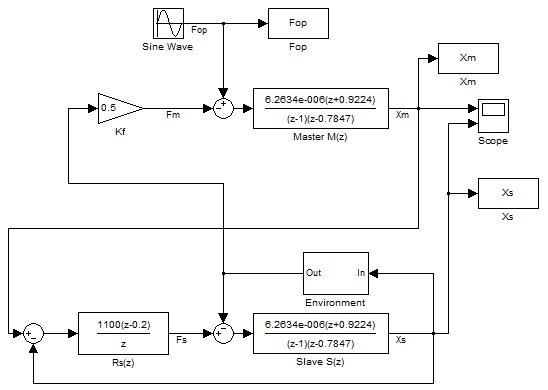
\includegraphics[width=10cm]{force-pos-esq}
	\caption{Esquema de control Fuerza - Posición en Simulink}
  	\label{fig:force-pos-esq}
\end{figure}
En la figura \ref{fig:force-pos-sim} se muestran los resultados obtenidos para los casos extremos que se han planteado.
\begin{figure}[htbp]
\centering
	\begin{subfigure}[h]
		\centering
		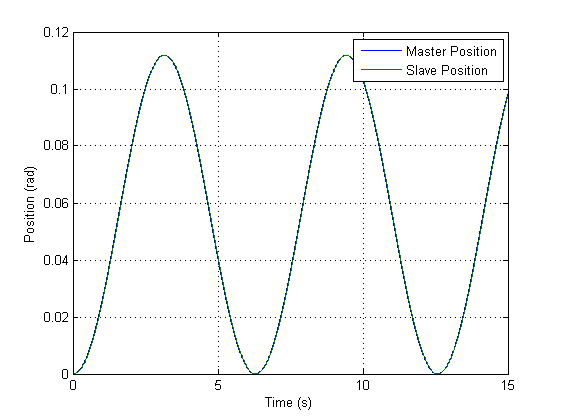
\includegraphics[height=5.25cm]{force-pos-libre}
		\caption{$K_e = 0$, entrada sinusoidal}
	\end{subfigure}
	\begin{subfigure}[h]
		\centering
		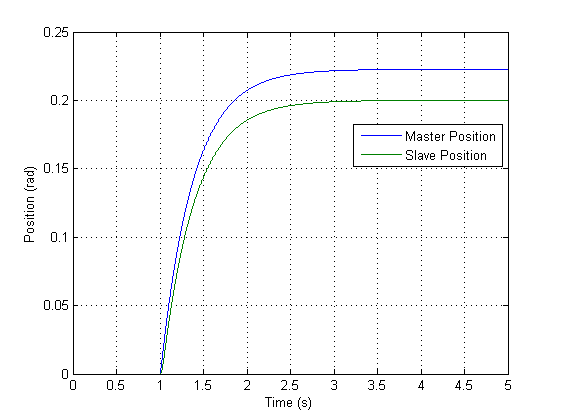
\includegraphics[height=5.25cm]{force-pos-env}
		\caption{$K_e = 100$, entrada escalón unitario}
	\end{subfigure}
	\caption{Simulación del control Fuerza - Posición}
  	\label{fig:force-pos-sim}
\end{figure}

\subsection{Experimentos}
\label{sub:force-pos-exp}
\begin{figure}[htbp]
\centering
	\begin{subfigure}[h]
		\centering
		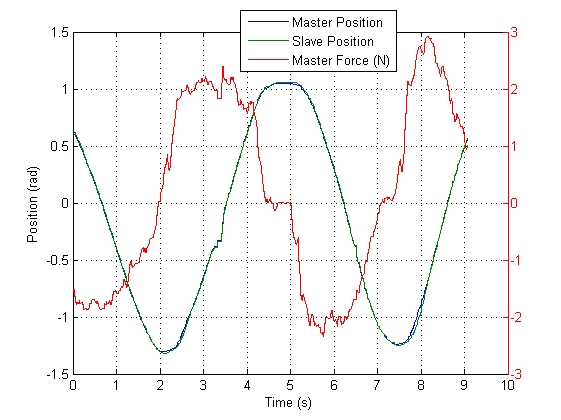
\includegraphics[height=5.25cm]{force-pos-exp-libre}
		\caption{Movimiento libre}
		\label{fig:force-pos-exp-libre}
	\end{subfigure}
	\begin{subfigure}[h]
		\centering
		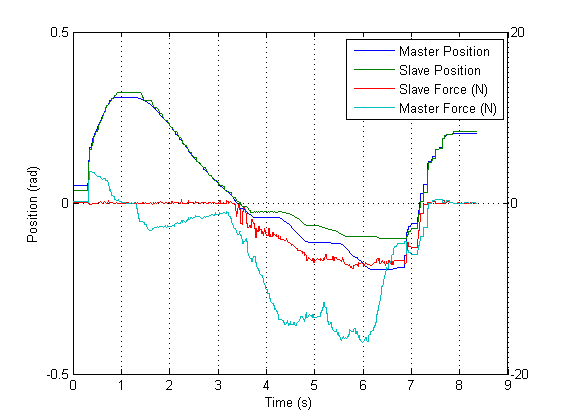
\includegraphics[height=5.25cm]{force-pos-exp-env}
		\caption{Colisión contra objeto rígido (t $\simeq$ 4-7 s. )}
		\label{fig:force-pos-exp-env}
	\end{subfigure}
	\caption{Resultados experimentales del control Fuerza - Posición}
  	\label{fig:force-pos-exp}
\end{figure}

Con el regulador diseñado se han realizado experimentos para comprobar el funcionamiento del sistema.
\begin{itemize}
\item Movimiento libre: En la figura \ref{fig:force-pos-exp-libre} se muestra como en el movimiento libre el maestro y el esclavo tienen la misma posición con error prácticamente nulo. Respecto a la fuerza percibida por el operador se aprecia que a pesar de estar en movimiento libre es necesario realizar hasta 3N para modificar la posición del sistema, aunque si se compara con el caso del control Posición - Posición (Numeral \ref{sub:pos-pos-exp}) el rango de posiciones alcanzadas es mayor.
\item Colisión: En la figura \ref{fig:force-pos-exp-env} se puede observar como durante el periodo de tiempo comprendido entre 4 y 7 segundos hay un error significativo en la posición. Además por la lectura de fuerza se puede ver que el pico de fuerza realizado por el operador alcanza los 17N y por otro lado la fuerza realizada por el esclavo en el entorno no supera los 8N.
\end{itemize}

\section{Arquitectura de Cuatro Canales}
\label{sec:4canales}
\begin{figure}[htbp]
\centering
	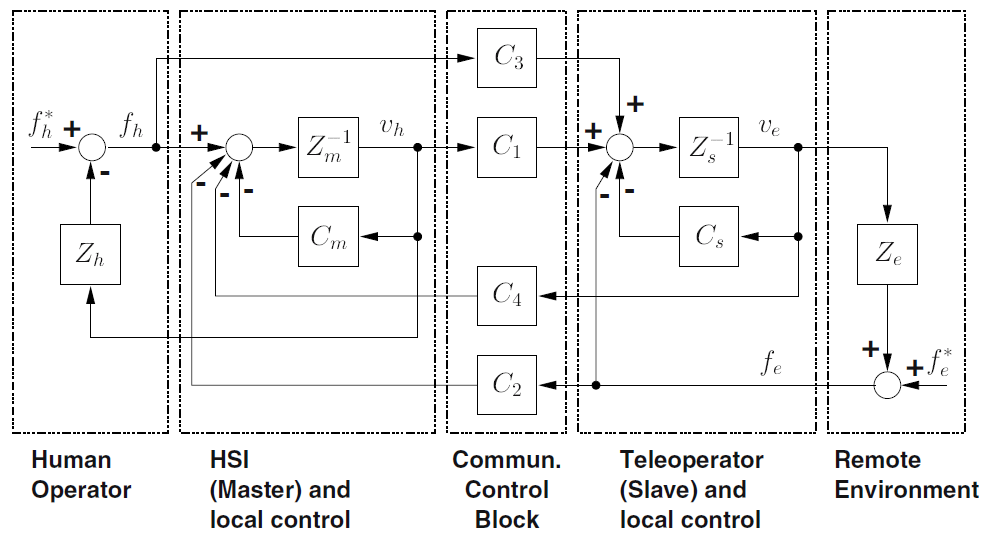
\includegraphics[width=\textwidth]{four}
	\caption{Arquitectura de control de 4 Canales} % labelInTOC
  	\label{fig:four} %% label for entire figure
\end{figure}
En esta sección se presentan los resultados obtenidos al utilizar la arquitectura de cuatro canales (figura \ref{fig:four}) en la plataforma experimental de la figura \ref{fig:setup}.
\begin{figure}[htbp]
\centering
	\begin{subfigure}[h]
		\centering
		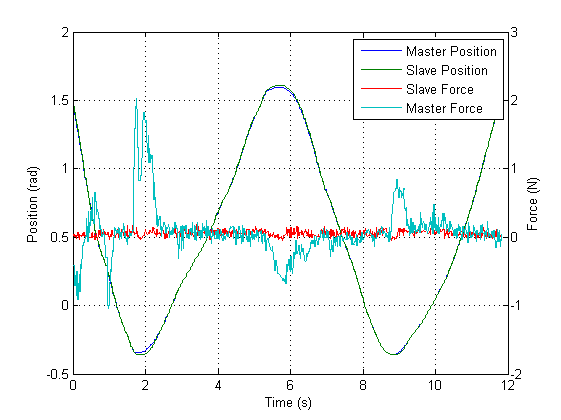
\includegraphics[height=5.25cm]{four-exp-libre}
		\caption{Movimiento  libre}
		\label{fig:four-exp-libre}
	\end{subfigure}
	\begin{subfigure}[h]
		\centering
		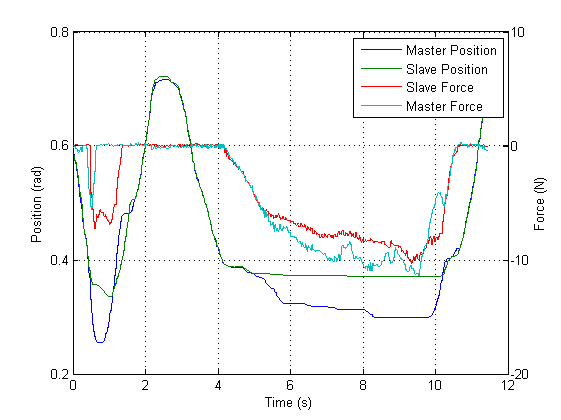
\includegraphics[height=5.25cm]{four-exp-env}
		\caption{Colisiones en $t\simeq 0-1.5$ s. y $t\simeq 5-10$ s.}
		\label{fig:four-exp-env}
	\end{subfigure}		
	\caption{Resultados experimentales de la Arquitectura de Cuatro Canales}
  	\label{fig:four-exp}
\end{figure}

Se han realizado experimentos en los casos extremos que se han mencionado anteriormente:
\begin{itemize}
\item Movimiento libre ($Z_e = 0$): En la figura \ref{fig:four-exp-libre} se muestra como en el movimiento libre el maestro y el esclavo tienen la misma posición con error prácticamente nulo. Respecto a la fuerza que el operador debe realizar para modificar la posición del sistema, se aprecia que tan solo es necesario aplicar fuerza cuando se cambia la dirección del movimiento y aún así la fuerza requerida es del orden de 1N. Si se comparan estos resultados con aquellos obtenidos con Posición - Posición (Fig. \ref{fig:pos-pos-exp-libre}) y con Fuerza - Posición (Fig. \ref{fig:force-pos-exp-libre}) salta a la vista que la arquitectura de cuatro canales permite una mejor percepción del entorno.

\item Colisión ($Z_e = \infty$): En la figura \ref{fig:four-exp-env} se muestran los resultados de dos colisiones con un entorno rígido. En $t\simeq 0-1.5$ seg. se puede advertir que la colisión se ha realizado a una velocidad elevada, con lo cual el sistema permite un error de posición elevado y a la hora de corregir se presenta una oscilación. Por otra parte, en $t\simeq 5-10$ seg., se observa una colisión a baja velocidad y en la que el operador realiza un fuerza sostenida sobre el maestro. Es interesante observar como la fuerza que realiza el esclavo sobre el entorno es trasmitida de manera casi exacta al operador, con lo cual se puede afirmar que para este caso extremo la arquitectura de cuatro canales también ofrece un mejor percepción del entorno en comparación con Posición - Posición (Fig. \ref{fig:pos-pos-exp-env}) y con Fuerza - Posición (Fig. \ref{fig:force-pos-exp-env}).
\end{itemize}

\section{Control por Convergencia de Estados}
\label{sec:convergencia}
\begin{figure}[htbp]
\centering
	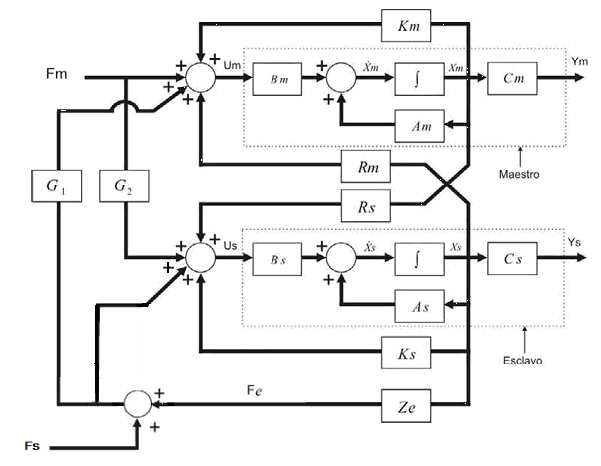
\includegraphics[height=8cm]{converge}
	\caption{Control por Convergencia de Estados}
  	\label{fig:converge}
\end{figure}
En esta sección se presentan los resultados obtenidos al utilizar el control por convergencia de estados (figura \ref{fig:converge}) en la plataforma experimental de la figura \ref{fig:setup}.
\begin{figure}[htbp]
\centering
	\begin{subfigure}[h]
		\centering
		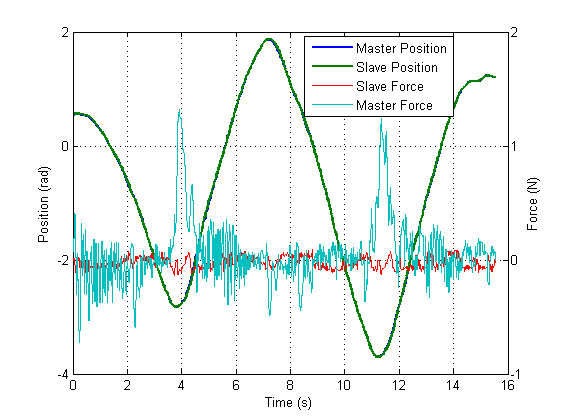
\includegraphics[width=\textwidth]{converge-exp-libre}
		\caption{Movimiento libre}
		\label{fig:converge-exp-libre}
	\end{subfigure}
	\begin{subfigure}[h]
		\centering
		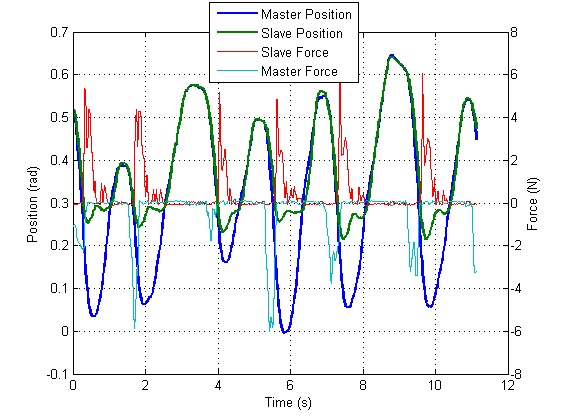
\includegraphics[width=\textwidth]{converge-exp-env}
		\caption{Colisiones contra objeto rígido}
		\label{fig:converge-exp-env}
	\end{subfigure}		
	\caption{Resultados experimentales del control por Convergencia de Estados}
  	\label{fig:converge-exp}
\end{figure}

Se han realizado experimentos en los casos extremos que se han mencionado anteriormente:
\begin{itemize}
\item Movimiento libre ($Z_e = 0$): En la figura \ref{fig:converge-exp-libre} se muestra como en el movimiento libre el maestro y el esclavo tienen la misma posición con error prácticamente nulo. Respecto a la fuerza que el operador debe realizar para modificar la posición del sistema, se aprecia que tan solo es necesario aplicar fuerza cuando se cambia la dirección del movimiento y aún así la fuerza requerida es del orden de 1N. Si se comparan estos resultados con aquellos obtenidos con la arquitectura de cuatro canales (Fig. \ref{fig:four-exp-libre}) salta a la vista que la percepción del entorno es similar pero debido a que tanto el maestro como el esclavo están constantemente corrigiendo el error el sistema es muy sensible al ruido en la medida de la fuerza.

\item Colisión ($Z_e = \infty$): En la figura \ref{fig:converge-exp-env} se muestran los resultados de varias colisiones con un entorno rígido. Todas las colisiones son a alta velocidad y la percepción del entorno es buena por parte del operador tal como lo demuestran las medidas de fuerza. Con respecto a los resultados obtenidos con la arquitectura de cuatro canales (Fig. \ref{fig:four-exp-env}) se puede decir que se el control por convergencia de estados se comporta mejor en colisiones en velocidad pero aún así el ruido que inducen los sensores de fuerza en la arquitectura hacen que la estabilidad del sistema se vea afectada.
\end{itemize}